\documentclass{article}
\usepackage{times}
% \usepackage[pdftex]{graphicx}
\usepackage{amsmath,amssymb,amsopn,amstext,amsfonts}
\usepackage{cancel}
\usepackage[space]{cite}
\usepackage{pdfsync}
\usepackage{bm}
\usepackage{balance}
\usepackage{color}
\usepackage{mathtools}
\usepackage{algpseudocode}
\usepackage{algorithm}
\newtheorem{theorem}{Theorem}
\usepackage{diagbox}
\usepackage{float}
\usepackage{epstopdf}
\usepackage{booktabs}
\usepackage{graphicx}
\usepackage{subfigure}
\usepackage{threeparttable}  
\usepackage{geometry}
\usepackage[utf8]{inputenc}
\usepackage{xeCJK}
\usepackage{setspace}
\geometry{a4paper,left=2cm,right=2cm,top=2cm,bottom=2cm}
\renewcommand{\figurename}{图}
\renewcommand{\tablename}{表}
\author{姓名:郭筠陶 \qquad 班级:自动化82 \qquad 学号:2181311665}
\renewcommand{\today}{\number\year 年 \number\month 月 \number\day 日}

\title{电子钟实验报告}
\begin{document}
\begin{spacing}{1.5}
    \maketitle
    本项目主要由如下模块组成:

    首先,通过对输入的24M Hz时钟信号进行24K分频,得到1KHz的时钟信号。
    然后对1K的时钟信号进行分频,得到1Hz的时钟信号。

    在当且仅当在计数到0的时候输出一个高电平,上升沿作为下一级(秒数的十位)的时钟信号输入。
    利用模6计数器和模10计数器各两个,组成一个异步时序电路,完成对分、秒的十位个位数字的计数。

    第二个模10计数器的输出信号作为时钟信号输入到一个模24计数器当中,模24计数器记录了小时数。
    由于24的个位不能看成是一个模10计数器,故不能像秒数、分数那样通过两个计数器来分别记录十位和个位的数字。
    而是需要通过一个转换单元,将模24的数字转换成十位和个位两个数字。

    1kHz的时钟信号输入到一个模6计数器当中,计数器的状态作为多路选择器的控制信号输入。
    计数器的值为0到5时分别对应时分秒中的共六位数字。

    上文中的两个模6计数器、两个模10计数器的状态,和转换器输出的小时数的两位数字,作为数据信号输入到多路选择器中。
    多路选择器会根据控制信号,来输出对应的数字。同时输出一个对应的片选信号。

    最终通过一个二进制数字到数码管代码的转化器,输出需要的七段管数据信号。

    同时,通过接入一个异步复位信号,使电子钟可以快进到23时59分59秒或其他任意事先指定的时间。
    \begin{figure}[H]
        \centering
        \includegraphics[width=4in]{mod24K.jpg}
        \caption{24K分频计数器代码}
    \end{figure}
    
    \begin{figure}[H]
        \centering
        \includegraphics[width=4in]{mod1K.jpg}
        \caption{1K分频计数器代码}
    \end{figure}

    \begin{figure}[H]
        \centering
        \includegraphics[width=4in]{mod6.jpg}
        \caption{六分频计数器代码}
    \end{figure}
    
    \begin{figure}[H]
        \centering
        \includegraphics[width=4in]{mod10.jpg}
        \caption{十分频计数器代码}
    \end{figure}

    \begin{figure}[H]
        \centering
        \includegraphics[width=4in]{mod24.jpg}
        \caption{24分频计数器代码}
    \end{figure}

    \begin{figure}[H]
        \centering
        \includegraphics[width=4in]{mod24_2_bcd.jpg}
        \caption{将0-23的二进制数提取出十位和个位的代码}
    \end{figure}
    
    \begin{figure}[H]
        \centering
        \includegraphics[width=4in]{multiplexer.jpg}
        \caption{多路选择器代码}
    \end{figure}

    \begin{figure}[H]
        \centering
        \includegraphics[width=4in]{eight_code.jpg}
        \caption{数码管输出代码}
    \end{figure}

    \begin{figure}
        \centering
        \includegraphics[width=4in]{circuit.jpg}
        \caption{电路连接图}
    \end{figure}

    \begin{figure}[H]
        \centering
        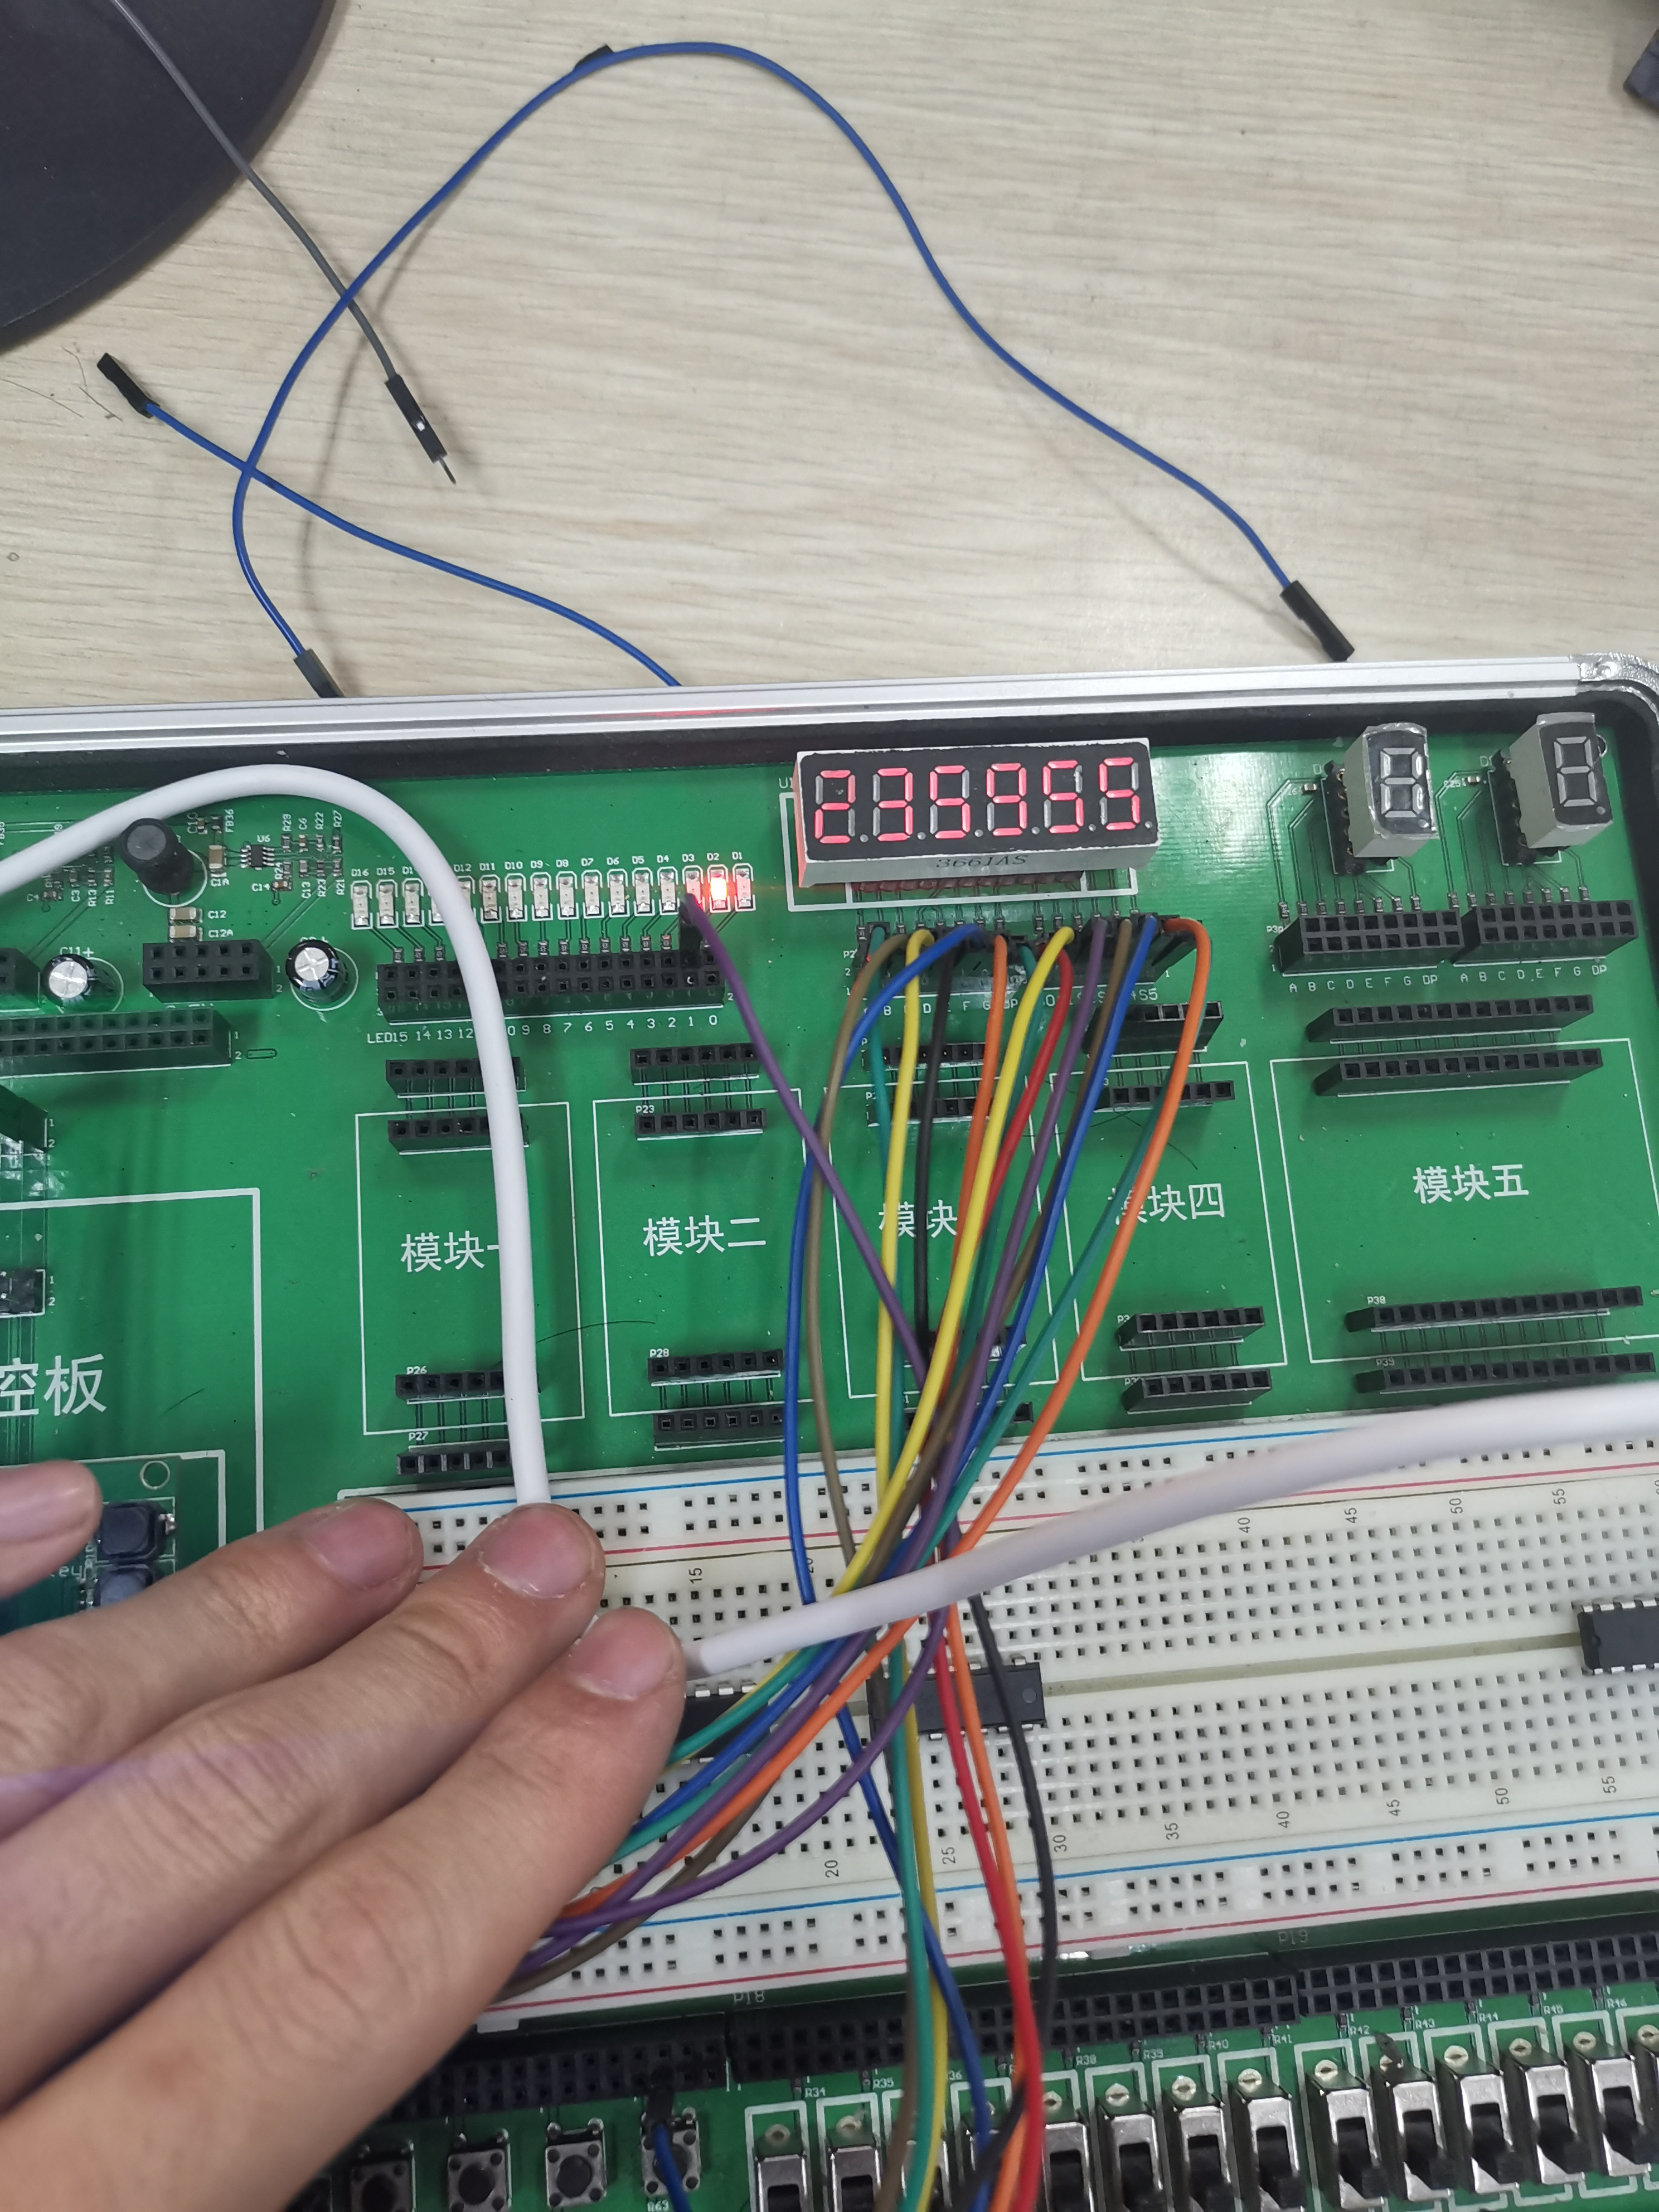
\includegraphics[width=4in]{final_result.jpg}
        \caption{最终电子钟显示效果}
    \end{figure}
\end{spacing}
\end{document}